\documentclass[11pt,a4paper]{article}
\emergencystretch=2em
\usepackage{graphicx}
\usepackage[T1]{fontenc}
\usepackage{lmodern,microtype,xcolor,geometry,amsmath,amssymb,amsthm,booktabs}
\usepackage[colorlinks=true,linkcolor=teal,citecolor=teal,urlcolor=teal]{hyperref}
\geometry{margin=27mm}
\makeatletter\g@addto@macro{\UrlBreaks}{\do\_}\makeatother
\newtheorem{theorem}{Theorem}
\newtheorem{lemma}[theorem]{Lemma}
\newtheorem{proposition}[theorem]{Proposition}
\newtheorem{corollary}[theorem]{Corollary}
\newtheorem{conjecture}[theorem]{Conjecture}
\theoremstyle{definition}
\newtheorem{claim}{Claim}
\newtheorem{remark}[theorem]{Remark}
\newcommand{\eps}{\varepsilon}
\newcommand{\diam}{\operatorname{diam}}
\newcommand{\dist}{\operatorname{dist}}
\newcommand{\R}{\mathbb R}
\title{The sharp upper edge of the normalised distance Laplacian}
\author{Anonymous\\[3pt]{\small DOI \href{https://doi.org/10.5281/zenodo.24540994}{10.5281/zenodo.24540994}}}
\date{November 2026}
\begin{document}
\maketitle
\begin{abstract}
The normalised distance Laplacian of a connected graph is the Laplacian of the random walk that moves from a vertex to another with probability proportional to their distance. Its eigenvalues lie in $[0,2]$, and the largest one is close to $2$ exactly when the walk nearly alternates between two regions. Reinhart conjectured that the maximum of this largest eigenvalue over graphs of order $n$ tends to $2$, and Johnston and Tait, who proved that limit, asked for the order of magnitude of the gap from $2$. We show that the gap is $4/\sqrt{3n}+o(n^{-1/2})$. Any sequence of graphs attaining this rate looks, at the scale of its diameter, like a path of length $(\sqrt3+o(1))\sqrt n$ with half of the vertices crowded at each end into nearly complete subgraphs; this description holds up to changes that are small at that scale, so it does not decide the exact maximiser. The same argument gives the sharp constant for every fixed positive power of the distance, for trees (where it is $4\sqrt{2/3}$ at power one), and for graphs excluding a fixed subgraph that contains a cycle. It also yields the limiting shape of the extremal eigenvector, shows that all other eigenvalues collapse to one, and identifies how the answer changes for regularly varying and for bounded distance weights. Exhaustive computations confirm that two stars joined by a path maximise the largest eigenvalue among all trees with at most twenty vertices.
\end{abstract}

\section{Introduction}
This section explains the question, what was known, what is new, and how the paper is organised.

\paragraph{The question.}
Let $G$ be a finite connected simple graph on $n$ vertices and let $d(u,v)$ be the number of edges in a shortest path from $u$ to $v$. Consider the random walk on the vertices that, from $u$, moves to $v\ne u$ with probability proportional to $d(u,v)$. Unlike the ordinary random walk on $G$, which moves only to neighbours, this walk prefers distant vertices. Its transition matrix is $P=T^{-1}\mathcal D$, where $\mathcal D$ is the distance matrix and $T$ is the diagonal matrix of row sums (the \emph{transmissions}). The matrix $L=I-T^{-1/2}\mathcal DT^{-1/2}$ is the \emph{normalised distance Laplacian}, introduced by Reinhart~\cite{reinhart}. It is symmetric and similar to $I-P$, so its eigenvalues are $1-\lambda$ for the eigenvalues $\lambda\in[-1,1]$ of $P$. In particular the largest eigenvalue (the spectral radius) of $L$ is
\[
\rho(G)=1-\lambda_{\min}(P)\in(1,2).
\]
It is close to $2$ when $P$ has an eigenvalue close to $-1$, that is, when the walk nearly alternates between two parts of the graph, like a chain of period two. The deficit $\eps(G)=2-\rho(G)$ measures how far the walk is from such alternation.

\paragraph{What was known.}
Reinhart computed the maximiser of $\rho$ for all graphs with at most ten vertices~\cite[Table~2.1]{reinhart}. She conjectured that the maximum over graphs of order $n$ tends to $2$ and that it is attained by two cliques joined by a path~\cite[Conjecture~2.10]{reinhart}. Johnston and Tait~\cite{jt} proved that the maximum tends to $2$. More precisely, their results give constants $c,C>0$ with
\[
 \frac cn\le\min_{|V(G)|=n}\eps(G)\le\frac C{\sqrt n};
\]
the upper bound comes from two cliques of about $n/2$ vertices joined by a path of about $\sqrt{2n}$ vertices, and, as they remark after their Proposition~4.2, this gives $C=2^{3/2}+o(1)=2\sqrt2+o(1)$ \cite{jt}. They also showed that the minimum deficit has order $n^{-1/2}$ under any one of three extra conditions on the extremal eigenvector \cite[Theorem~4.7]{jt}. In the last paragraph of their Section~4 they note that a proof of Reinhart's conjecture seems difficult and that it would be interesting even to determine the order of magnitude of $\min\eps$. Other work on this matrix concerns its smallest positive eigenvalue: Byrne, Johnston, Schildkraut and Tait~\cite{bjst} bounded it below and conjectured the bound $2/3$, which Kumar and Patra~\cite{kp} proved in the sharp form $2/3+4/(3t_{\max})$. See also the survey~\cite{hr}. The analogous extremal problem for the ordinary random walk was solved by Aksoy, Chung, Tait and Tobin~\cite{aksoy}; there the extremal graphs also consist of dense ends joined by a path, but the operator, the extremal power of $n$ and the proof differ.

\paragraph{What is new.}
We determine the minimum deficit to first order, with no condition on the eigenvector:
\[
 \min_{|V(G)|=n}\eps(G)=\frac{4}{\sqrt{3n}}+o\big(n^{-1/2}\big)\qquad(4/\sqrt3\approx2.3094).
\]
Every sequence of graphs that attains this rate has a shortest path of length $(\sqrt3+o(1))\sqrt n$ which every vertex is close to, at the scale of that length, and half of the vertices sit near each end in nearly complete subgraphs (Theorem~\ref{th:specific}). The improvement from $2\sqrt2$ to $4/\sqrt3$ in the construction comes from letting the eigenvector interpolate linearly along the path instead of vanishing there. The method extends to the weights $d(u,v)^\alpha$ for every fixed $\alpha>0$, to trees, to graphs without a fixed subgraph containing a cycle (Theorem~\ref{th:main} and Corollary~\ref{cor:forbidden}), and to regularly varying and bounded weights (Section~\ref{sec:weights}). For near-extremal graphs it gives the limiting shape of the extremal eigenvector and shows that all eigenvalues of $L$ other than $0$ and $\rho$ collapse to $1$ in mean square (Corollary~\ref{cor:spectrum}). Finally, exhaustive computations show that among trees with at most twenty vertices the maximiser is always two stars whose centres are joined by a path (Section~\ref{sec:finite}), which suggests a tree analogue of Reinhart's conjecture.

\paragraph{What is not settled.}
The result is first order. Graphs that differ from two cliques joined by a path by $o(n^2)$ edges inside the ends, or by branches of length $o(\sqrt n)$, have the same leading deficit, so the theorem does not decide Reinhart's exact conjecture. Numerically the best clique--path--clique graph has deficit about $4/\sqrt{3n}-4.26/n$ at $n=10^6$ (Table~\ref{tab:kpk}); a matching lower bound at order $1/n$ would be the natural next step.

\paragraph{Idea of the proof.}
The lower bound has three steps. First, we look at the eigenvector $y$ of the smallest eigenvalue of $P$ at its maximum and minimum vertices $i$ and $j$. Because $P$ nearly reverses the sign of $y$, the rows of $P$ at $i$ and $j$ can share very little probability; this is the classical Doeblin--Dobrushin contraction bound~\cite{gq} applied to two chosen rows. It forces almost all vertices to lie very close to $i$ or to $j$, compared with $d(i,j)$. Second, on these two clusters $y$ is nearly $+1$ and $-1$, and the Rayleigh quotient splits into a cost inside the clusters, which prefers a long separation, and a cost from the vertices of a shortest $i$--$j$ path, which prefers a short one. Third, each path vertex can choose its eigenvector value, but at best it pays a definite amount computed from a one-variable quadratic; adding these amounts and optimising the separation gives the constant. The matching construction places two balanced dense blocks at the ends of a path of the optimal length.

\paragraph{Organisation.}
Section~\ref{sec:setting} fixes notation and the variational formula for the deficit. Section~\ref{sec:results} states the main theorems and says where each part is proved. Section~\ref{sec:overlap} proves the row-overlap inequality and its first consequences. Section~\ref{sec:lower} proves the sharp lower bound and Section~\ref{sec:construction} the matching constructions. Section~\ref{sec:stability} derives the structure of near-extremal graphs, and Section~\ref{sec:forbidden} treats forbidden subgraphs and trees. Section~\ref{sec:spectrum} describes the rest of the spectrum and the extremal eigenvector. Section~\ref{sec:weights} treats other distance weights. Section~\ref{sec:finite} reports finite computations, and Section~\ref{sec:discussion} discusses limits and open problems.

\section{Setting and notation}\label{sec:setting}
This section defines the operator for a general distance power and rewrites the deficit as a minimum of a ratio of two quadratic forms.

Throughout, $G=(V,E)$ is a connected simple graph of order $n\ge3$, $d(u,v)$ is graph distance and $D_G=\diam(G)$ (we write $D$ when $G$ is clear). Fix $\alpha>0$ and put
\[
 W_{uv}=d(u,v)^\alpha\ (u\ne v),\quad W_{uu}=0,\quad t_u=\sum_v W_{uv},\quad T=\mathrm{diag}(t_u),\quad P=T^{-1}W,
\]
\[
 L_\alpha=I-T^{-1/2}WT^{-1/2},\qquad \rho_\alpha(G)=\lambda_{\max}(L_\alpha),\qquad \eps(G)=2-\rho_\alpha(G)=1+\lambda_{\min}(P).
\]
At $\alpha=1$ this is Reinhart's matrix, and we write $\rho=\rho_1$. The matrix $P$ is stochastic and reversible, and it is similar to the symmetric matrix $T^{-1/2}WT^{-1/2}$.

For $y\in\R^V$ define the \emph{energy} and the \emph{weight}
\[
 E(y)=\sum_{\{u,v\}}W_{uv}(y_u+y_v)^2,\qquad Z(y)=\sum_u t_u y_u^2=\sum_{\{u,v\}}W_{uv}(y_u^2+y_v^2),
\]
where every sum over $\{u,v\}$ runs over unordered pairs of distinct vertices. Writing $x=T^{1/2}y$, one has $x^{\mathsf T}(I+T^{-1/2}WT^{-1/2})x=E(y)$ and $x^{\mathsf T}x=Z(y)$, so by the Rayleigh principle
\begin{equation}\label{eq:var}
 \eps(G)=\min_{y\ne0}\frac{E(y)}{Z(y)},
\end{equation}
and a minimiser satisfies $Py=(-1+\eps)y$. We call such a $y$ an \emph{extremal eigenvector}. Since $P$ has trace zero and eigenvalue one, its smallest eigenvalue is negative, so $0\le\eps<1$.

Two scales appear throughout:
\[
 h=h_n=n^{1/(1+\alpha)},\qquad \varrho=\varrho_n=h_n^{1/2}.
\]
The first is the length of the optimal path; the second is a radius, small compared with $h$, used to define the two dense clusters. Table~\ref{tab:notation} collects the symbols used in the proofs.

\begin{table}[ht]
\centering\small
\begin{tabular}{ll}
\toprule
Symbol & Meaning\\\midrule
$W,\ t_u,\ P$ & distance weights $d^\alpha$, transmissions, transition matrix\\
$\eps(G)$ & deficit $2-\rho_\alpha(G)=1+\lambda_{\min}(P)$\\
$E(y),\ Z(y)$ & energy and weight in \eqref{eq:var}\\
$y,\ i,\ j,\ \mu$ & extremal eigenvector scaled so $y_i=\max y=1$; $j$ a minimum vertex, $\mu=y_j\ge-1$\\
$r,\ Q$ & $r=d(i,j)$; $Q=(v_0=i,\dots,v_r=j)$ a fixed shortest $i$--$j$ path\\
$h,\ \varrho$ & scales $n^{1/(1+\alpha)}$ and $h^{1/2}$\\
$A,\ B$ & the two \emph{cores}: vertices near $i$ (resp.\ $j$) where $y$ is near $+1$ (resp.\ $-1$)\\
$p,\ q$ & limiting core fractions $|A|/n$, $|B|/n$\\
$s$ & limiting scaled separation $r/h$\\
$U(S)$ & internal cost $\sum_{\{u,v\}\subset S}d(u,v)^\alpha$ of a vertex set $S$\\
$b$ & class constant (Section~\ref{sec:results})\\
$C_\alpha,\ s_*,\ K_{\alpha,b}$ & constants of Theorem~\ref{th:main}\\
\bottomrule
\end{tabular}
\caption{Notation used in Sections~\ref{sec:overlap}--\ref{sec:spectrum}.}\label{tab:notation}
\end{table}

\section{Main results}\label{sec:results}
This section states the sharp asymptotic for Reinhart's matrix, its generalisation to distance powers and restricted classes, and a map of where each part is proved.

\begin{theorem}\label{th:specific}
Let $M_n$ be the maximum of $\rho(G)$ over connected simple graphs of order $n$. Then
\[
 \lim_{n\to\infty}\sqrt n\,(2-M_n)=\frac4{\sqrt3}.
\]
Let $(G_n)$ be any sequence of connected graphs of order $n$ with $\sqrt n\,(2-\rho(G_n))\to4/\sqrt3$. Then:
\begin{enumerate}
\item[(a)] $\diam(G_n)=(\sqrt3+o(1))\sqrt n$;
\item[(b)] there are disjoint vertex sets $A_n,B_n$, each of size $(1/2+o(1))n$, whose induced subgraphs have edge density tending to one;
\item[(c)] with distances divided by the diameter and the uniform probability measure on vertices, $G_n$ converges in the measured Gromov--Hausdorff sense (defined in Section~\ref{sec:stability}) to the interval $[0,1]$ carrying the measure $\frac12\delta_0+\frac12\delta_1$.
\end{enumerate}
\end{theorem}

The limit space in (c) is the whole interval, while the limit measure sits on its two endpoints: the path is metrically visible although it carries a vanishing fraction of the vertices.

To state the general result, consider one of three classes $\mathcal C$ of connected graphs: all connected simple graphs; connected $K_{\kappa+1}$-free graphs for a fixed $\kappa\ge2$; or trees. The class enters only through a constant $b$, the smallest possible asymptotic mean of $d^\alpha$ over pairs inside a large vertex set:
\[
\begin{array}{c|ccc}
\mathcal C & \text{all graphs}&K_{\kappa+1}\text{-free graphs}&\text{trees}\\ \hline
 b &1&1+(2^\alpha-1)/\kappa&2^\alpha
\end{array}
\]
Define
\begin{equation}\label{eq:constants}
 C_\alpha=4\int_0^1\frac{z^\alpha(1-z)^\alpha}{z^\alpha+(1-z)^\alpha}\,dz,\qquad
 s_*=\Big(\frac{2\alpha b}{C_\alpha}\Big)^{1/(1+\alpha)},\qquad
 K_{\alpha,b}=2b s_*^{-\alpha}+C_\alpha s_* .
\end{equation}
The number $K_{\alpha,b}$ is the minimum over $s>0$ of $2bs^{-\alpha}+C_\alpha s$, attained only at $s_*$. In this sum, $2bs^{-\alpha}$ is the cost of pairs inside the two dense ends and $C_\alpha s$ the cost of pairs between the path and the ends, for a path of length $sh_n$.

\begin{theorem}\label{th:main}
Fix $\alpha>0$ and one of the three classes. Then
\[
 \lim_{n\to\infty} h_n^\alpha\min_{G\in\mathcal C,\ |V(G)|=n}\eps(G)=K_{\alpha,b}.
\]
If $G_n\in\mathcal C$ has order $n$ and $h_n^\alpha\eps(G_n)\to K_{\alpha,b}$, then $G_n$ has a shortest path of length $(s_*+o(1))h_n$ such that every vertex is within distance $o(h_n)$ of it, and two disjoint sets of $(1/2+o(1))n$ vertices that lie within distance $o(h_n)$ of its two endpoints, respectively. In each of these sets the mean of $d(u,v)^\alpha$ over unordered pairs of distinct vertices tends to $b$.
\end{theorem}

At $\alpha=1$ one has $C_1=4\int_0^1z(1-z)\,dz=2/3$, $s_*=\sqrt{3b}$ and $K_{1,b}=4\sqrt{b/3}$. This gives $4/\sqrt3\approx2.3094$ for all graphs, $4\sqrt{(1+1/\kappa)/3}$ for $K_{\kappa+1}$-free graphs and $4\sqrt{2/3}\approx3.2660$ for trees. (For triangle-free graphs at $\alpha=1$ the constant is $2\sqrt2$, numerically equal to the Johnston--Tait barbell constant for all graphs; this is a coincidence of two different trade-offs.)

\paragraph{Where the proofs are.}
The lower bound $\liminf h_n^\alpha\min\eps\ge K_{\alpha,b}$ is Proposition~\ref{prop:lower} (Section~\ref{sec:lower}), which rests on Lemmas~\ref{lem:overlap} and~\ref{lem:coarse} (Section~\ref{sec:overlap}). The matching upper bound is Proposition~\ref{prop:construction} (Section~\ref{sec:construction}). The structural statements of Theorem~\ref{th:main} are proved in Section~\ref{sec:stability}. Theorem~\ref{th:specific} is the case $\alpha=1$, $b=1$: the limit is $K_{1,1}=4/\sqrt3$; part~(a) is \eqref{eq:diam}; part~(b) is Proposition~\ref{prop:stability}(iii) with $b=1$; part~(c) is proved at the end of Section~\ref{sec:stability}.

\section{The row-overlap inequality}\label{sec:overlap}
This section shows that the two rows of $P$ at the extreme vertices of an extremal eigenvector overlap very little, and deduces the coarse size of the diameter and of the separation $r$.

Let $y$ be an extremal eigenvector. Replacing $y$ by $-y$ if necessary and scaling, we may assume $y_i=\max_u y_u=1$ for a vertex $i$ and $\mu=y_j=\min_u y_u\ge-1$ for a vertex $j$. The eigen-equation at $i$ reads $\sum_xP_{ix}y_x=-1+\eps$; since the left side is at least $\mu$, we get $\mu\le-1+\eps$.

\begin{lemma}\label{lem:overlap}
With this normalisation,
\begin{equation}\label{eq:two}
 \sum_x W_{ix}(1+y_x)=\eps\,t_i,\qquad \sum_x W_{jx}(1-y_x)\le2\eps\,t_j,
\end{equation}
and
\begin{equation}\label{eq:overlap}
 \sum_x\min(W_{ix},W_{jx})\le\eps\max(t_i,t_j).
\end{equation}
\end{lemma}
\begin{proof}
The first identity is the eigen-equation at $i$ multiplied by $t_i$. At $j$, $(Py)_j=(-1+\eps)\mu=(1-\eps)|\mu|\ge(1-\eps)^2$, because $|\mu|\ge1-\eps$. Hence $\sum_xP_{jx}(1-y_x)=1-(Py)_j\le1-(1-\eps)^2\le2\eps$, which is the second inequality.

For \eqref{eq:overlap}, let $a_x=\min(P_{ix},P_{jx})$. Writing $P_{ix}=a_x+\pi_x$ and $P_{jx}=a_x+\pi'_x$ with $\pi,\pi'\ge0$ and $\sum\pi_x=\sum\pi'_x=1-\sum a_x$, the common part cancels in $(Py)_i-(Py)_j$ and the rest is a difference of two averages of values in $[\mu,1]$. Hence
\[
 (1-\eps)(1-\mu)=(Py)_j-(Py)_i\le(1-\mu)\Big(1-\sum_xa_x\Big),
\]
where the equality uses $(Py)_i=(-1+\eps)\cdot1$ and $(Py)_j=(-1+\eps)\mu$. Since $1-\mu>0$, this gives $\sum_xa_x\le\eps$. Finally $a_x\ge\min(W_{ix},W_{jx})/\max(t_i,t_j)$.
\end{proof}

The inequality $\sum_x a_x\le\eps$ is the statement that every eigenvalue $\lambda\ne1$ of a stochastic matrix satisfies $|\lambda|\le1-\min_{u,v}\sum_x\min(P_{ux},P_{vx})$, the Doeblin--Dobrushin ergodicity coefficient bound (see \cite[equations (1)--(2)]{gq}), applied to the two rows that matter (a left eigenvector for $\lambda\ne1$ has zero sum, and the coefficient is the norm of $P$ on zero-sum vectors). We claim no novelty for it; what is used below is the freedom to choose the rows at the extremes of $y$.

\begin{lemma}\label{lem:coarse}
With $c_\alpha=1/(3\cdot8^\alpha)$, every connected graph of order $n\ge3$ satisfies
\[
 \eps(G)\ge c_\alpha\max\{D^{-\alpha},\,D/n\},\qquad D=\diam(G).
\]
If $\eps(G)\le K_0h_n^{-\alpha}$ for a constant $K_0$, then $D$ and $r=d(i,j)$ are both between two positive constant multiples of $h_n$ (depending on $\alpha$ and $K_0$), and
\begin{equation}\label{eq:radial}
 \sum_x\min\big(d(i,x),d(j,x)\big)^\alpha\le\eps\max(t_i,t_j)\le C_0\,n
\end{equation}
for a constant $C_0=C_0(\alpha,K_0)$.
\end{lemma}
\begin{proof}
In \eqref{eq:overlap} every vertex $x\ne i,j$ contributes $\min(W_{ix},W_{jx})\ge1$ to the left side, while $\max_ut_u\le nD^\alpha$. Thus $\eps\ge(n-2)/(nD^\alpha)\ge D^{-\alpha}/3$.

For the second bound, fix a diametral shortest path $R$ with $D+1$ vertices. Two vertices of $R$ are at graph distance equal to their separation along $R$, so a ball of integer radius $l$ contains at most $2l+1$ vertices of $R$ (its first and last vertices on $R$ are at distance at most $2l$). Let $D\ge8$ and $l=\lfloor D/8\rfloor$. At least $D+1-2(2l+1)\ge D/3$ vertices of $R$ lie outside both balls of radius $l$ about $i$ and $j$, and each contributes at least $(l+1)^\alpha\ge(D/8)^\alpha$ to the left side of \eqref{eq:overlap}. Hence $\eps\ge(D/3)(D/8)^\alpha/(nD^\alpha)=D/(3\cdot8^\alpha n)$. For $D<8$ the first bound already gives $\eps\ge8^{-\alpha}/3\ge D/(3\cdot 8^\alpha n)$ because $D\le n$. This proves the first assertion.

Now suppose $\eps\le K_0h^{-\alpha}$. The bound $\eps\ge D^{-\alpha}/3$ gives $D\ge(3K_0)^{-1/\alpha}h$, and $\eps\ge c_\alpha D/n$ gives $D\le K_0 n h^{-\alpha}/c_\alpha=K_0h/c_\alpha$. Since $\max(t_i,t_j)\le nD^\alpha$, \eqref{eq:overlap} gives \eqref{eq:radial} with $C_0=K_0(K_0/c_\alpha)^\alpha$. Equation~\eqref{eq:overlap} also gives $\max(t_i,t_j)\ge(n-2)/\eps\ge(n-2)h^\alpha/K_0$. On the other hand, for every $x$, $\max(d(i,x),d(j,x))\le r+\min(d(i,x),d(j,x))$, and $(a+c)^\alpha\le2^{\alpha}(a^\alpha+c^\alpha)$ for $a,c\ge0$, so by \eqref{eq:radial} $\max(t_i,t_j)\le2^{\alpha}(nr^\alpha+C_0n)$. Comparing the two bounds shows $r\ge c'h$ for some $c'>0$ and all large $n$. Finally $r\le D$.
\end{proof}

\section{The sharp lower bound}\label{sec:lower}
This section proves that no graph in the class can have scaled deficit below $K_{\alpha,b}$, by splitting the energy into the costs inside two dense cores and between the cores and a shortest path.

\begin{proposition}\label{prop:lower}
For each of the three classes, $\liminf_{n\to\infty}h_n^\alpha\min_{G\in\mathcal C,|V(G)|=n}\eps(G)\ge K_{\alpha,b}$. More precisely, let $G_n\in\mathcal C$ with $h_n^\alpha\eps(G_n)\le K_0$, and pass to a subsequence along which $r/h_n\to s$, $|A|/n\to p$ and $|B|/n\to q$ (with $A,B$ the cores constructed below). Then $s>0$, $p+q=1$, $p,q>0$ and
\begin{equation}\label{eq:key}
 \liminf h_n^\alpha\eps(G_n)\ \ge\ b\,\frac{p^2+q^2}{pq}\,s^{-\alpha}+2I_\alpha(p)\,s
 \ \ge\ 2b s^{-\alpha}+C_\alpha s\ \ge\ K_{\alpha,b},
\end{equation}
where $I_\alpha(p)=\int_0^1\frac{z^\alpha(1-z)^\alpha}{pz^\alpha+q(1-z)^\alpha}\,dz$. Equality in the middle inequality forces $p=q=1/2$, and equality in the last forces $s=s_*$.
\end{proposition}

It suffices to consider sequences with $h_n^\alpha\eps(G_n)\le K_0$, since otherwise there is nothing to prove; by Lemma~\ref{lem:coarse}, $r/h_n$ is bounded above and below, so a further subsequence has $r/h_n\to s\in(0,\infty)$. The proof consists of four claims. All $o(\cdot)$ and $O(\cdot)$ symbols refer to $n\to\infty$ along the subsequence, with constants depending only on $\alpha$, $K_0$ and the class. Note that $r\asymp h=o(n)$ and $\varrho=h^{1/2}=o(r)$.

\begin{claim}[Covering by two balls]\label{cl:cover}
Let $B_i$ and $B_j$ be the balls of radius $\varrho$ about $i$ and $j$. They are disjoint for large $n$, and at most $C_0n/\varrho^\alpha=o(n)$ vertices lie outside $B_i\cup B_j$.
\end{claim}
\begin{proof}
Disjointness holds since $r>2\varrho$ eventually. A vertex outside both balls contributes more than $\varrho^\alpha$ to the left side of \eqref{eq:radial}.
\end{proof}

\begin{claim}[Near-constancy on the cores]\label{cl:cores}
$\sum_{x\in B_i}(1-y_x)=O(\eps n)$ and $\sum_{x\in B_j}(1+y_x)=O(\eps n)$. Consequently, if $A$ consists of the vertices $x\in B_i\setminus Q$ with $1-y_x\le h^{-\alpha/2}$ and $B$ of the vertices $x\in B_j\setminus Q$ with $1+y_x\le h^{-\alpha/2}$, then $|V\setminus(A\cup B)|=o(n)$, and $|y_x-1|\le h^{-\alpha/2}$ on $A$, $|y_x+1|\le h^{-\alpha/2}$ on $B$.
\end{claim}
\begin{proof}
All terms in the second relation of \eqref{eq:two} are nonnegative because $y\le1$. For $x\in B_i$, $d(j,x)\ge r-\varrho$, so $W_{jx}\ge(r-\varrho)^\alpha$, and therefore
\[
 \sum_{x\in B_i}(1-y_x)\le\frac{2\eps t_j}{(r-\varrho)^\alpha}\le\frac{2\eps nD^\alpha}{(r-\varrho)^\alpha}=O(\eps n),
\]
using $D=O(r)$. The bound on $B_j$ follows in the same way from the first relation of \eqref{eq:two}, whose terms are nonnegative because $y\ge-1$. By Markov's inequality at most $O(\eps n)h^{\alpha/2}=O(nh^{-\alpha/2})=o(n)$ vertices of $B_i\cup B_j$ exceed the threshold $h^{-\alpha/2}$. The path $Q$ has $r+1=o(n)$ vertices. Together with Claim~\ref{cl:cover}, this proves the count.
\end{proof}

Call the $o(n)$ vertices outside $A\cup B$ \emph{exceptional}. Within $A$ (or $B$) all distances are at most $2\varrho=o(r)$, and for $x\in A$, $x'\in B$ we have $|d(x,x')-r|\le2\varrho$.

\begin{claim}[The weight]\label{cl:weight}
$Z(y)=(2pq+o(1))\,n^2r^\alpha$.
\end{claim}
\begin{proof}
Use $Z(y)=\sum_{\{u,v\}}W_{uv}(y_u^2+y_v^2)$. Pairs $\{x,x'\}$ with $x\in A$, $x'\in B$ have $W=(1+o(1))r^\alpha$ and $y_x^2+y_{x'}^2=2+o(1)$, uniformly; there are $|A||B|=(pq+o(1))n^2$ of them. Pairs inside $A$ or inside $B$ number at most $n^2$, each with $W\le(2\varrho)^\alpha=o(r^\alpha)$ and $y^2\le1$. Pairs with an exceptional vertex number $o(n)\cdot n$, each with $W\le D^\alpha=O(r^\alpha)$.
\end{proof}

For a vertex set $S$ write $U(S)=\sum_{\{u,v\}\subset S}d(u,v)^\alpha$ for its internal cost.

\begin{claim}[Three disjoint energy contributions]\label{cl:energy}
Let $\mathcal C$ be one of the three classes and $b$ its constant.
\begin{enumerate}
\item[(i)] For every vertex set $S$ of a graph in $\mathcal C$ with $|S|=m$,
\begin{equation}\label{eq:intra}
 U(S)\ge b\binom m2-O(m).
\end{equation}
\item[(ii)] The pairs inside $A$ and inside $B$ contribute at least $(2b(p^2+q^2)-o(1))n^2$ to $E(y)$.
\item[(iii)] If $p,q>0$, the pairs $\{v_l,x\}$ with $v_l\in Q$ and $x\in A\cup B$ contribute at least $(4pqI_\alpha(p)-o(1))\,nr^{1+\alpha}$ to $E(y)$.
\end{enumerate}
The pair sets in (ii) and (iii) are disjoint, because $A$, $B$ and $Q$ are disjoint.
\end{claim}
\begin{proof}
(i) Distinct vertices have distance at least $1$, which gives the case $b=1$. In a $K_{\kappa+1}$-free graph, the subgraph induced on $S$ is $K_{\kappa+1}$-free and so, by Tur\'an's theorem (recalled in the introduction of \cite{es}), has at most $(1-1/\kappa)m^2/2$ edges; all other pairs in $S$ are at distance at least $2$. Hence $U(S)\ge2^\alpha\binom m2-(2^\alpha-1)(1-1/\kappa)\frac{m^2}2=b\binom m2-O(m)$. In a tree at most $m-1$ pairs of $S$ are adjacent and the rest are at distance at least $2$, so $U(S)\ge2^\alpha\binom m2-(2^\alpha-1)(m-1)$.

(ii) For $u,v\in A$, $(y_u+y_v)^2\ge(2-2h^{-\alpha/2})^2=4-o(1)$, and similarly on $B$. By (i) the contribution is at least $(4-o(1))\big(U(A)+U(B)\big)\ge(4-o(1))\,b\,\big(\binom{|A|}2+\binom{|B|}2\big)-O(n)=(2b(p^2+q^2)-o(1))n^2$.

(iii) Fix $l\in\{0,\dots,r\}$, put $z=l/r$, $\omega=y_{v_l}\in[-1,1]$, $a=z^\alpha$ and $c=(1-z)^\alpha$. For $x\in A$, $|d(x,v_l)-l|\le d(x,i)\le\varrho$, so $d(x,v_l)/r=z+O(\varrho/r)$; since $u\mapsto u^\alpha$ is uniformly continuous on $[0,2]$, $W_{v_lx}=r^\alpha(a+o(1))$ uniformly in $l$ and $x$. Likewise $W_{v_lx}=r^\alpha(c+o(1))$ for $x\in B$. Moreover $(y_x+\omega)^2=(1+\omega)^2+O(h^{-\alpha/2})$ on $A$ and $(y_x+\omega)^2=(1-\omega)^2+O(h^{-\alpha/2})$ on $B$, uniformly because $|\omega|\le1$. Therefore, uniformly in $l$,
\[
 \sum_{x\in A\cup B}W_{v_lx}(y_x+\omega)^2=nr^\alpha\big\{pa(1+\omega)^2+qc(1-\omega)^2+o(1)\big\}.
\]
For fixed $a,c\ge0$ with $pa+qc>0$, the quadratic $\omega\mapsto pa(1+\omega)^2+qc(1-\omega)^2$ has minimum $4pqac/(pa+qc)$ (at $\omega=(qc-pa)/(pa+qc)$). The function $z\mapsto 4pq\,ac/(pa+qc)$ is continuous on $[0,1]$, because $pa+qc\ge\min(p,q)\min_z(z^\alpha+(1-z)^\alpha)>0$. Summing over $l$ and comparing with a Riemann sum gives at least $nr^\alpha\big(4pq\,r\,I_\alpha(p)-o(r)\big)$.
\end{proof}

\begin{proof}[Proof of Proposition~\ref{prop:lower}]
Since $A$ and $B$ together contain all but $o(n)$ vertices, $p+q=1$. Suppose $pq=0$. By Claim~\ref{cl:weight}, $Z(y)=o(n^2r^\alpha)$, while Claim~\ref{cl:energy}(ii) gives $E(y)\ge(2b(p^2+q^2)-o(1))n^2\ge(b-o(1))n^2$. Then $h^\alpha\eps=h^\alpha E(y)/Z(y)\to\infty$ because $r\asymp h$, contrary to assumption. Hence $p,q>0$.

Dividing the sum of the two lower bounds of Claim~\ref{cl:energy} by Claim~\ref{cl:weight}, and using $n=h^{1+\alpha}$ and $r/h\to s$,
\[
 h^\alpha\eps=\frac{h^\alpha E(y)}{Z(y)}\ \ge\ \frac{2b(p^2+q^2)}{2pq}\Big(\frac hr\Big)^\alpha+\frac{4pqI_\alpha(p)}{2pq}\cdot\frac{r}{h}-o(1),
\]
which is the first inequality in \eqref{eq:key}. For the second, $(p^2+q^2)/(pq)\ge2$ with equality only at $p=q$. Substituting $z\mapsto1-z$ in $I_\alpha(p)$ exchanges $a$ and $c$, so
\[
 2I_\alpha(p)=\int_0^1ac\Big(\frac1{pa+qc}+\frac1{pc+qa}\Big)dz\ \ge\ \int_0^1\frac{4ac}{(p+q)(a+c)}\,dz=C_\alpha,
\]
by $1/X+1/Y\ge4/(X+Y)$. The last inequality in \eqref{eq:key} is the definition of $K_{\alpha,b}$: the function $s\mapsto 2bs^{-\alpha}+C_\alpha s$ is strictly convex with its unique minimum at $s_*$.
\end{proof}

\section{Constructions attaining the bound}\label{sec:construction}
This section exhibits, in each class, graphs whose deficit attains the lower bound to first order.

\begin{proposition}\label{prop:construction}
For each of the three classes, $\limsup_{n\to\infty}h_n^\alpha\min_{G\in\mathcal C,|V(G)|=n}\eps(G)\le K_{\alpha,b}$.
\end{proposition}
\begin{proof}
Choose integers $r=r_n$ with $r/h_n\to s_*$, and two blocks $S_1,S_2$ of sizes $m_1,m_2$ differing by at most one with $m_1+m_2+r-1=n$. For all graphs, make each block a clique; for $K_{\kappa+1}$-free graphs, a complete $\kappa$-partite graph with parts as equal as possible; for trees, a star. Choose one vertex in each block (the centre, for a star) and join the two chosen vertices by a path with $r$ edges and $r-1$ new internal vertices $v_1,\dots,v_{r-1}$; write $v_0,v_r$ for the chosen vertices. The resulting graph is connected and lies in its class (complete $\kappa$-partite graphs and paths contain no $K_{\kappa+1}$). Each block has diameter at most $2$, and as $|S|\to\infty$ its internal cost satisfies $U(S)=(b+o(1))\binom{|S|}2$: for the $\kappa$-partite block, a fraction $1/\kappa+o(1)$ of pairs lie in a common part (distance $2$) and the rest are adjacent.

Define the trial vector $y=1$ on $S_1$, $y=-1$ on $S_2$, and on internal path vertices
\[
 y_{v_l}=\frac{(1-z)^\alpha-z^\alpha}{(1-z)^\alpha+z^\alpha},\qquad z=l/r.
\]
We bound $E(y)$ and $Z(y)$ by groups of pairs. Pairs between the two blocks have $y_u+y_v=0$ and contribute no energy. Pairs inside the blocks contribute $4\big(U(S_1)+U(S_2)\big)=(b+o(1))n^2$. For a path vertex at $z=l/r$, its distances to block vertices are $l+O(1)$ and $r-l+O(1)$, so the computation in Claim~\ref{cl:energy}(iii), now with $p=q=1/2$ and the pointwise minimising value of $\omega$, shows that block-to-path pairs contribute $(I_\alpha(1/2)+o(1))\,nr^{1+\alpha}=(C_\alpha/2+o(1))\,nr^{1+\alpha}$, because $I_\alpha(1/2)=2\int_0^1ac/(a+c)\,dz=C_\alpha/2$. Path-to-path pairs contribute $O(r^{2+\alpha})=o(n^2)$, because $r^{1+\alpha}\asymp n$ and $r=o(n)$. Finally $Z(y)=(1/2+o(1))n^2r^\alpha$, by the argument of Claim~\ref{cl:weight} with $p=q=1/2$. Using $n=h^{1+\alpha}$,
\[
 h^\alpha\eps\le\frac{h^\alpha E(y)}{Z(y)}=\frac{(b+o(1))n^2+(C_\alpha/2+o(1))\,nr^{1+\alpha}}{(1/2+o(1))\,n^2r^\alpha}\,h^\alpha
 =2b\Big(\frac hr\Big)^\alpha+C_\alpha\frac rh+o(1)\longrightarrow K_{\alpha,b}.
\]
\end{proof}

No assumption on the true eigenvector enters this construction: the trial vector gives an upper bound on $\eps$ through \eqref{eq:var}. Figure~\ref{fig:balance} illustrates the trade-off at $\alpha=1$.

\begin{figure}[ht]
\centering
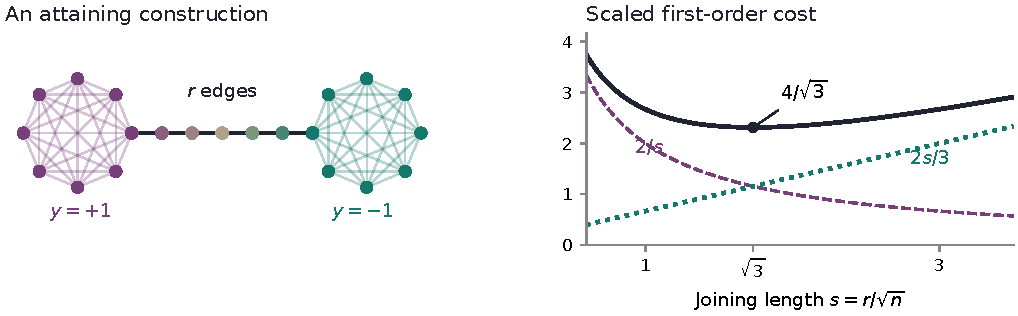
\includegraphics[width=.95\linewidth]{figures/distance-balance.pdf}
\caption{Left: the unrestricted construction (two cliques joined by a path); the colour of a path vertex indicates its trial value, which falls linearly from $+1$ to $-1$ at $\alpha=1$. Right: the limiting scaled deficit at $\alpha=1$ for a joining path of $r=s\sqrt n$ edges. Pairs inside the cliques contribute $2/s$ and path-to-clique pairs contribute $2s/3$; the sum is smallest at $s=\sqrt3$, where it equals $4/\sqrt3$. The drawing shows the construction at a small order.}\label{fig:balance}
\end{figure}

\section{Structure of near-extremal graphs}\label{sec:stability}
This section shows that a sequence attaining the sharp constant must have balanced cores, the optimal separation, and no long branches away from the path; it then proves the metric limit in Theorem~\ref{th:specific}(c).

Throughout, $G_n\in\mathcal C$ with $h_n^\alpha\eps(G_n)\to K_{\alpha,b}$, and $y,i,j,r,Q,A,B$ are as in Section~\ref{sec:lower}.

\begin{proposition}\label{prop:stability}
Under this assumption:
\begin{enumerate}
\item[(i)] $|A|/n\to1/2$, $|B|/n\to1/2$ and $r/h_n\to s_*$ along the full sequence;
\item[(ii)] every vertex is within distance $o(r)$ of $Q$, and $r\le\diam(G_n)\le r+o(r)$;
\item[(iii)] $U(A)=(b+o(1))\binom{|A|}2$ and $U(B)=(b+o(1))\binom{|B|}2$; for $b=1$ the induced edge densities of $A$ and $B$ tend to one.
\end{enumerate}
\end{proposition}
\begin{proof}
(i) Along any subsequence where the limits $p,q,s$ exist, \eqref{eq:key} holds with left side $K_{\alpha,b}$, so all its inequalities are equalities: $p=q=1/2$ and $s=s_*$. Every subsequence has a further subsequence with limits, and the limits are always the same, so the full sequence converges.

(iii) Since the limits in \eqref{eq:key} are attained, the counted energy of Claim~\ref{cl:energy}, $E_{\rm count}$, satisfies $E(y)-E_{\rm count}=o(n^2)$, and each of the two counted parts is within $o(n^2)$ of its lower bound. In particular $4(1-o(1))(U(A)+U(B))\le(b+o(1))n^2$. Combined with \eqref{eq:intra} for $A$ and for $B$ separately, this gives the two asymptotics. For $b=1$, each nonadjacent pair adds at least $2^\alpha-1$ to its baseline cost $1$, so the number of nonadjacent pairs in $A$ is $o(n^2)$; the same holds in $B$.

(ii) Suppose that along a subsequence some vertex $u$ has $\dist(u,Q)=\ell_n\ge\delta r$ for a fixed $\delta>0$. Take the first $\lfloor\ell_n/2\rfloor$ vertices on a shortest path from $u$ to $Q$. Each is at distance at least $\ell_n/2$ from $Q$, hence at distance at least $\ell_n/2-\varrho$ from $A\cup B$ (every core vertex is within $\varrho$ of an endpoint of $Q$). These vertices lie outside $A$, $B$ and $Q$, so their pairs with core vertices are not counted in $E_{\rm count}$. For such a vertex $u'$ with value $\omega=y_{u'}$, $\sum_{x\in A\cup B}(y_{u'}+y_x)^2\ge|A|((1+\omega)^2-o(1))+|B|((1-\omega)^2-o(1))\ge(1-o(1))n\min_\omega\tfrac12[(1+\omega)^2+(1-\omega)^2]=(1-o(1))n$. Each of these pairs has weight at least $(\ell_n/2-\varrho)^\alpha$. Hence the uncounted energy is at least $c\,n\,\ell_n^{1+\alpha}\ge c\,n(\delta r)^{1+\alpha}$, which is of order $n^2$ because $r^{1+\alpha}\asymp n$. This contradicts $E(y)-E_{\rm count}=o(n^2)$. Therefore $\max_u\dist(u,Q)=o(r)$, and by the triangle inequality
\begin{equation}\label{eq:diam}
 r\le\diam(G_n)\le r+o(r)=(s_*+o(1))h_n.
\end{equation}
\end{proof}

Proposition~\ref{prop:stability} proves the structural statements of Theorem~\ref{th:main}: $Q$ is the required shortest path, and $A$, $B$ are the required sets (within distance $\varrho=o(h)$ of the endpoints of $Q$, with mean internal cost tending to $b$ by (iii)).

\paragraph{The metric limit.}
We use the following standard notion. Compact metric spaces $(X_n,d_n)$ with Borel probability measures $\nu_n$ are said to converge in the \emph{measured Gromov--Hausdorff sense} to $(X,d,\nu)$ if there are maps $\phi_n:X_n\to X$ such that $\sup_{u,v}|d(\phi_n u,\phi_n v)-d_n(u,v)|\to0$, every point of $X$ is within $o(1)$ of $\phi_n(X_n)$, and the push-forward measures $\phi_{n\#}\nu_n$ converge weakly to $\nu$. The limit space $X$ is kept in full even when the limit measure has smaller support.

\begin{proof}[Proof of Theorem~\ref{th:specific}(c)]
Let $d_n=d/\diam(G_n)$ and $\nu_n$ be uniform on $V(G_n)$. Map each vertex $u$ to $\phi_n(u)=l/r$, where $v_l$ is a nearest vertex of $Q$ to $u$. Since every vertex is within $o(r)$ of $Q$ and $Q$ is a shortest path, $|d(u,v)-r|\phi_n(u)-\phi_n(v)||=o(r)$ for all $u,v$; with \eqref{eq:diam} this gives distortion $o(1)$ for $d_n$. The image contains $\{l/r\}$, which is $1/r$-dense in $[0,1]$. All vertices of $A$ map into $[0,o(1)]$ and all vertices of $B$ into $[1-o(1),1]$, and these sets carry fractions $1/2+o(1)$ of the vertices. Hence $\phi_{n\#}\nu_n\to\frac12\delta_0+\frac12\delta_1$ weakly.
\end{proof}

\section{Forbidden subgraphs and the structure of extremal trees}\label{sec:forbidden}
This section extends the class of graphs to those excluding any fixed subgraph with a cycle and describes near-extremal trees exactly up to $o(n)$ edits.

\begin{corollary}\label{cor:forbidden}
Let $F$ be a fixed graph containing a cycle and put $\kappa=\chi(F)-1\ge1$. For connected $F$-free graphs (graphs with no subgraph isomorphic to $F$), Theorem~\ref{th:main} holds with $b=1+(2^\alpha-1)/\kappa$. If $\kappa\ge2$, each of the two sets $A,B$ of a near-extremal sequence can be made a complete $\kappa$-partite graph by $o(n^2)$ edge changes. For trees, an asymptotically extremal sequence can be turned into two stars whose centres are joined by a path by $o(n)$ edge changes.
\end{corollary}
\begin{proof}
Since $F$ is a subgraph of the complete $(\kappa+1)$-partite graph with parts of size $|V(F)|$, the Erd\H os--Stone theorem~\cite{es} shows that an $F$-free graph on $m$ vertices has at most $(1-1/\kappa+o(1))m^2/2$ edges. This replaces the $O(m)$ error in \eqref{eq:intra} by $o(m^2)$, which is all that Claim~\ref{cl:energy}(ii) and Proposition~\ref{prop:stability} use. For $\kappa\ge2$ the constructions of Proposition~\ref{prop:construction} are $\kappa$-colourable and therefore $F$-free. For $\kappa=1$ ($F$ bipartite with a cycle) the tree construction is $F$-free because trees have no cycles, and $b=2^\alpha$ is the tree constant. When $\kappa\ge2$, Proposition~\ref{prop:stability}(iii) forces each set $A$, $B$ to have $(1-1/\kappa-o(1))|A|^2/2$ edges (resp.\ for $B$), and the Erd\H os--Simonovits stability theorem, in the form proved by F\"uredi~\cite{furedi}, gives the edit statement. (For $\kappa=1$ and $F$-free graphs that are not trees we make no structural claim.)

For trees, let $S$ be one of the two sets and $m=|S|$. Only $m-1$ pairs of $S$ are adjacent, so $U(S)=(2^\alpha+o(1))\binom m2$ forces all but $o(m^2)$ pairs to be at distance exactly two. Write $a_v=|N(v)\cap S|$ for each vertex $v$ of the tree. Two vertices at distance two in a tree have a unique common neighbour, so $\sum_va_v(a_v-1)\ge(1-o(1))m^2$. Consider the bipartite graph with one copy of $S$ on one side, the vertices $v$ with $a_v\ge2$ on the other, and an edge for each adjacency of the tree. It is a subgraph of the bipartite double cover of the tree, which is two disjoint copies of the tree, so it is a forest and has at most $m+\#\{v:a_v\ge2\}-1$ edges. Hence $\sum_v(a_v-1)_+\le m-1$. Since $\sum_va_v(a_v-1)\le\max_va_v\cdot\sum_v(a_v-1)_+$, we get $\max_va_v\ge(1-o(1))m$: some hub is adjacent to all but $o(m)$ vertices of $S$. The hubs of the two sets are within $\varrho+1$ of the respective endpoints of $Q$, so they are distinct and far apart. Keep the tree path between the hubs and the edges from each hub to its neighbours in its own set; this is a subtree on $n-o(n)$ vertices consisting of a path and two stars. Deleting the $o(n)$ remaining edges of the tree and attaching each of the $o(n)$ remaining vertices to a hub gives two stars joined by a path, after $o(n)$ edge changes.
\end{proof}

\section{The remaining spectrum and the extremal eigenvector}\label{sec:spectrum}
This section shows that, near the extremum, the matrix $P$ has essentially two nonzero eigenvalues, and it determines the extremal eigenvector everywhere to first order.

Write $0=\lambda_1\le\dots\le\lambda_n=\rho_\alpha$ for the eigenvalues of $L_\alpha$; the eigenvalues of $P$ are $1-\lambda_k$.

\begin{corollary}\label{cor:spectrum}
If $h_n^\alpha\eps(G_n)=O(1)$, then
\[
 \sum_{k=2}^{n-1}(1-\lambda_k)^2\longrightarrow0.
\]
If moreover $h_n^\alpha\eps(G_n)\to K_{\alpha,b}$, orient $Q$ from $i$ to $j$ and, for each vertex $u$, let $z_u\in[0,1]$ be $l/r$ for a nearest vertex $v_l$ of $Q$ to $u$. Then, uniformly over all vertices,
\[
 y_u=\frac{(1-z_u)^\alpha-z_u^\alpha}{(1-z_u)^\alpha+z_u^\alpha}+o(1).
\]
\end{corollary}
\begin{proof}
Pass to a subsequence along which $p$, $q$ and $s$ converge; by Proposition~\ref{prop:lower}, $p,q>0$. For every vertex $u$, one of $i,j$ is at distance at least $r/2$ from $u$, so at least $\min(|A|,|B|)\ge cn$ vertices are at distance at least $r/2-\varrho$ from $u$. Hence $\min_ut_u\ge c\,nr^\alpha$, and every entry of $P$ is $O(1/n)$ since $D=O(r)$. Now $\mathrm{tr}(P^2)=\sum_{u,v}P_{uv}P_{vu}=\sum_k(1-\lambda_k)^2$. Pairs involving an exceptional vertex contribute $o(n)\cdot n\cdot O(n^{-2})=o(1)$. Within a core, $P_{uv}=O(\varrho^\alpha/(nr^\alpha))=o(1/n)$, so these pairs contribute $o(1)$. For $u\in A$, $t_u=(q+o(1))nr^\alpha$ (cross-core pairs dominate, as in Claim~\ref{cl:weight}), and for $v\in B$, $t_v=(p+o(1))nr^\alpha$. Hence for $u\in A$, $v\in B$, $P_{uv}P_{vu}=(1+o(1))/(pqn^2)$, and the $2|A||B|$ ordered cross pairs contribute $2+o(1)$. So $\sum_k(1-\lambda_k)^2=2+o(1)$. The two extreme eigenvalues of $P$ are $1$ and $-1+\eps\to-1$, which account for $2+o(1)$; the remaining sum tends to zero. The limit does not depend on the subsequence.

For the second assertion, $p=q=1/2$ and every vertex is within $o(r)$ of $Q$ (Proposition~\ref{prop:stability}). Uniformly in $u$, $d(u,x)/r=z_u+o(1)$ for $x\in A$ and $d(u,x)/r=1-z_u+o(1)$ for $x\in B$. In the eigen-equation $(-1+\eps)y_u=\sum_xP_{ux}y_x$, the exceptional vertices contribute $o(1)$ because entries of $P$ are $O(1/n)$, and the cores contribute
\[
 \frac{z_u^\alpha-(1-z_u)^\alpha+o(1)}{z_u^\alpha+(1-z_u)^\alpha+o(1)}
\]
since $y=\pm1+o(1)$ on the cores and $t_u=\frac n2r^\alpha\big(z_u^\alpha+(1-z_u)^\alpha+o(1)\big)$. As $z^\alpha+(1-z)^\alpha\ge\min\{1,2^{1-\alpha}\}>0$ and $\eps\to0$, the profile follows.
\end{proof}

\section{Other distance weights}\label{sec:weights}
This section replaces the power $d^\alpha$ by a general nondecreasing weight and shows which features of the answer persist: for regularly varying weights of positive index everything carries over, at index zero the optimal path length is no longer determined, and for bounded weights the deficit no longer tends to zero.

Let $w$ be a nondecreasing function on the nonnegative integers with $w(0)=0$ and $w(1)>0$, and replace $W_{uv}=d(u,v)^\alpha$ by $W_{uv}=w(d(u,v))$. Denote the resulting deficit by $\eps_w$; formula \eqref{eq:var} and Lemma~\ref{lem:overlap} hold unchanged. A sequence of graphs is \emph{asymptotically minimising} if its deficit divided by the minimum over graphs of the same order and class tends to one.

\begin{theorem}\label{th:regular}
Suppose $w$ is unbounded and regularly varying with index $\alpha\ge0$, that is, $w(\lfloor zk\rfloor)/w(k)\to z^\alpha$ as $k\to\infty$ for every $z>0$. Define $h=\max\{k:kw(k)\le n\}$. For unrestricted graphs put $b=w(1)$, for trees $b=w(2)$, and for graphs excluding a fixed subgraph $F$ containing a cycle $b=w(1)+(w(2)-w(1))/(\chi(F)-1)$. In each of these classes
\[
 \lim_{n\to\infty} w(h)\min_{|V(G)|=n}\eps_w(G)
 =\begin{cases} K_{\alpha,b},&\alpha>0,\\2b,&\alpha=0.\end{cases}
\]
For $\alpha>0$, every asymptotically minimising sequence satisfies $\diam(G_n)/h\to s_*$ and has the path and balanced-core structure of Theorem~\ref{th:main}. For $\alpha=0$, every asymptotically minimising sequence has two vertices $i,j$ (the extremes of an extremal eigenvector) at distance $r$ with $r=o(h)$ and $w(r)\sim w(h)$, has $\diam(G_n)=o(h)$, and has $(1/2+o(1))n$ vertices within distance $o(r)$ of each of $i$ and $j$.
\end{theorem}

\begin{proof}
\emph{Preliminary facts about $w$.} Because $w$ is nondecreasing, the convergence $w(\lfloor zk\rfloor)/w(k)\to z^\alpha$ is uniform for $z$ in compact subsets of $(0,\infty)$: sandwich $z$ between consecutive points of a fine finite partition and use continuity of $z^\alpha$. In particular $w(k+1)/w(k)\to1$, so $hw(h)\sim n$ and $h=o(n)$. Taking $z=2$ shows that there is $C\ge1$ with $w(2k)\le Cw(k)$ for all $k\ge1$, and hence $w(a+c)\le C\,[w(a)+w(c)]$ for all integers $a,c\ge0$ (apply the doubling bound at $\max(a,c)$). When $\alpha>0$ the uniform convergence extends to $z\in(0,1]$ including the limit $z\downarrow0$: for $z\le\delta$ monotonicity gives $0\le w(\lfloor zk\rfloor)/w(k)\le w(\lfloor\delta k\rfloor)/w(k)\to\delta^\alpha$.

\emph{Coarse bounds.} It suffices for the lower bound to consider $\eps_w\le K_0/w(h)$. Inequality \eqref{eq:overlap} gives $\eps_w\ge(n-2)w(1)/(nw(D))$, so $w(D)\to\infty$ and $D\to\infty$. The ball argument of Lemma~\ref{lem:coarse} gives $\eps_w\ge c\,Dw(\lfloor D/8\rfloor)/(nw(D))\ge c'D/n$, by doubling. Thus $D=O(h)$ and $w(D)=O(w(h))$, and \eqref{eq:overlap} gives $\sum_xw(\min(d(i,x),d(j,x)))=O(n)$. As in Lemma~\ref{lem:coarse}, $\max(t_i,t_j)\ge(n-2)w(1)/\eps_w$ while $\max(t_i,t_j)=O(nw(r)+n)$ by doubling, so $w(r)\ge c\,w(h)$ and $r\to\infty$.

\emph{Cores at the new scale.} Repeat Claims~\ref{cl:cover}--\ref{cl:weight} with the core radius $\varrho=\lfloor\sqrt r\rfloor$ in place of $h^{1/2}$ and the discarding threshold $\eps_w^{1/2}$ in place of $h^{-\alpha/2}$. Because $w(\varrho)\to\infty$, at most $O(n)/w(\varrho)=o(n)$ vertices lie outside the two balls. On the ball about $i$, $w(d(j,x))\ge w(r-\varrho)=(1+o(1))w(r)$, so \eqref{eq:two} gives $\sum(1-y_x)=O(n\eps_w w(D)/w(r))=O(n\eps_w)$ there, and at most $O(n\eps_w^{1/2})=o(n)$ vertices exceed the threshold; similarly at $j$. Cross-core weights are $(1+o(1))w(r)$ uniformly. Exceptional pairs contribute $o(n^2w(r))$ to $Z(y)$ since $w(D)=O(w(r))$. Inside a core the largest weight need not be $o(w(r))$ when $\alpha=0$, but the \emph{total} internal weight is $O(n^2)=o(n^2w(r))$: for $x,x'$ in the ball about $i$, $w(d(x,x'))\le C(w(d(i,x))+w(d(i,x')))$, and $\sum_xw(d(i,x))$ over that ball is $O(n)$ by the radial bound. Hence, along any subsequence with core fractions $p,q$,
\[
 Z(y)=(2pq+o(1))n^2w(r),\qquad E_{\rm internal}\ge(2b(p^2+q^2)-o(1))n^2,
\]
where the second bound uses \eqref{eq:intra} with $w(1),w(2)$ in place of $1,2^\alpha$ (and Corollary~\ref{cor:forbidden} for $F$-free graphs). Since one core has linear size and $b>0$, bounded $w(h)\eps_w$ again forces $pq>0$.

\emph{Positive index.} If $\alpha>0$, then $w(r)\ge c\,w(h)$ and $r=O(h)$ force $r/h$ to stay away from zero (by the uniform convergence down to $z\downarrow0$), so along a subsequence $r/h\to s>0$ and $w(r)/w(h)\to s^\alpha$. Claim~\ref{cl:energy}(iii) holds with $w(r)$ in place of $r^\alpha$, using the uniform convergence on $[0,1]$, and the proof of Proposition~\ref{prop:lower} gives \eqref{eq:key}. The construction of Proposition~\ref{prop:construction} with $r/h\to s_*$ has the same costs, since block distances take only the values $1$ and $2$; path-to-path energy is $O(r^2w(r))=o(n^2)$. Equality forces $p=q=1/2$ and $s=s_*$, and the branch argument of Proposition~\ref{prop:stability}(ii) applies with uncounted energy of order $nhw(h)\asymp n^2$.

\emph{Index zero: lower bound.} Let $\alpha=0$. Along a subsequence put $s=\lim r/h\in[0,\infty)$ and $\tau=\lim w(r)/w(h)$; then $\tau>0$ by the coarse bounds and $\tau\le1$ because $r\le D=O(h)$ and $w$ is slowly varying and nondecreasing. For path vertices $v_l$ with $l/r\in[\eta,1-\eta]$, both $w(d(v_l,x))/w(r)$ for $x$ in either core tend to one uniformly, so each such vertex contributes at least $(4pq-o(1))\,nw(r)$ to its core interactions (the quadratic of Claim~\ref{cl:energy}(iii) with $a=c=1$). Summing over these $(1-2\eta)r$ vertices, dividing by $Z(y)$ and letting $\eta\downarrow0$,
\[
 \liminf w(h)\eps_w\ \ge\ b\,\frac{p^2+q^2}{pq\,\tau}+2s\ \ge\ 2b .
\]

\emph{Index zero: upper bound.} Choose integers $r=r_n\to\infty$ with $r=o(h)$ and $w(r)\sim w(h)$; for instance $r=\lfloor h/J\rfloor$ where $J=J(h)\to\infty$ slowly enough. (Explicitly, for fixed $J$ the ratio $w(\lfloor h/J\rfloor)/w(h)\to1$, so increase $J$ to $J+1$ only once $h/(J+1)\ge J+1$ and the ratio for $J+1$ is within $1/(J+1)$ of one for this and all larger $h$.) Join two balanced cliques by a path with $r$ edges and use the trial vector $+1$, $-1$ on the cliques and $0$ on internal path vertices. Block-to-path energy is $O(nrw(r+2))=o(n^2)$, path-to-path and cross-block energies vanish or are $o(n^2)$, internal energy is $(b+o(1))n^2$, and $Z(y)\ge(1/2+o(1))n^2w(r)$. This gives $\limsup w(h)\eps_w\le2b$ for every such choice of $r$. (For trees and $F$-free graphs use stars or balanced complete multipartite blocks.)

\emph{Index zero: structure.} Equality forces $p=q=1/2$, $\tau=1$ and $s=0$, so $r=o(h)$ and $w(r)\sim w(h)$, and $E_{\rm internal}$ accounts for $E(y)$ up to $o(n^2)$. If $D\ge\delta h$ along a subsequence, then, since $r=o(h)$, some vertex $u$ is at distance at least $\delta h/3$ from both $i$ and $j$. Following a shortest path from $u$ towards $\{i,j\}$ produces $\Omega(h)$ vertices outside the cores and at distance $\Omega(h)$ from both cores. Each has core interactions of at least $(1-o(1))\,n\,w(\Omega(h))\asymp nw(h)$, as in Proposition~\ref{prop:stability}(ii), giving $\Omega(nhw(h))=\Omega(n^2)$ uncounted energy, a contradiction. Hence $D=o(h)$. The core statement is Claim~\ref{cl:cover} at radius $\varrho=o(r)$.
\end{proof}

For example $w(d)=\log(1+d)$ gives $h\sim n/\log n$ and an unrestricted minimum deficit $(2\log2+o(1))/\log n$. Both $r=\lfloor n/(\log n)^2\rfloor$ and $r=\lfloor n/(\log n)^3\rfloor$ are asymptotically optimal joining lengths, although their ratio diverges.

\begin{corollary}\label{cor:bounded}
Suppose instead that $w(d)$ increases to a finite limit $w_\infty$ and write $w_1=w(1)>0$. Over unrestricted connected graphs of order $n$, the minimum deficit tends to $2w_1/(w_1+w_\infty)$.
\end{corollary}
\begin{proof}
We prove a finite inequality for any symmetric weight matrix with zero diagonal and off-diagonal entries in $[w_1,w_\infty]$. Put
\[
 f(a)=\frac{w_1(a-1)}{w_1(a-1)+w_\infty(n-a)},\qquad 1\le a\le n-1 .
\]
Every eigenvalue $\lambda\ne1$ of $P$ satisfies $1+\lambda\ge\min_{u\ne v}\sum_x\min(P_{ux},P_{vx})$ (the bound used in Lemma~\ref{lem:overlap}). For two rows $u\ne v$, let $S=\{x:P_{ux}>P_{vx}\}$ and $a=|S|$; then $v\in S$, $u\notin S$ and $\sum_x\min(P_{ux},P_{vx})=P_v(S)+P_u(V\setminus S)$. The row of $v$ puts weight at least $w_1$ on each of the $a-1$ points of $S\setminus\{v\}$ and at most $w_\infty$ on each of the $n-a$ points of $V\setminus S$, so $P_v(S)\ge f(a)$; likewise $P_u(V\setminus S)\ge f(n-a)$. The function $f$ is convex on $[1,n-1]$ (it is a constant plus a positive multiple of the reciprocal of a decreasing affine function, and linear when $w_1=w_\infty$), so $f(a)+f(n-a)\ge f(\lfloor n/2\rfloor)+f(\lceil n/2\rceil)$. The symmetric matrix with weight $w_1$ inside two groups of sizes $\lfloor n/2\rfloor,\lceil n/2\rceil$ and $w_\infty$ across attains this bound: its two-group quotient has eigenvalue $f(\lfloor n/2\rfloor)+f(\lceil n/2\rceil)-1$. As $n\to\infty$ the bound tends to $2w_1/(w_1+w_\infty)$.

For graphs, join two balanced cliques by a path whose length tends to infinity and is $o(n)$, and use the trial vector $+1$, $-1$ on the cliques and $0$ on the path. The internal energy is $(w_1+o(1))n^2$, path interactions cost $o(n^2)$, and $Z(y)=((w_1+w_\infty)/2+o(1))n^2$. This gives the matching upper bound.
\end{proof}
The limiting contrast $(w_\infty-w_1)/(w_\infty+w_1)=1-2w_1/(w_1+w_\infty)$ equals $\tanh(\Delta/4)$ with $\Delta=2\log(w_\infty/w_1)$; this is Birkhoff's classical bound on the contraction ratio, in Hilbert's projective metric, of any positive matrix with entries in $[w_1,w_\infty]$, since $\Delta$ bounds its projective diameter (Birkhoff's formula, see \cite[Theorem~5.6]{gq}). The corollary adapts it to zero diagonals at finite $n$ and shows that graph distances attain it.

\section{Finite computations}\label{sec:finite}
This section reports exact-enumeration and large-order computations at $\alpha=1$ that complement the asymptotic theorems; none of them is used in a proof.

The script \texttt{code/finite\_search.py} computes $\eps(G)=1+\lambda_{\min}(P)$ for every connected graph of order $4$ to $9$ and every tree of order $6$ to $20$ (generated by \texttt{geng} and \texttt{gentreeg} from nauty), and compares the minimum with the best member of the clique--path--clique family (for all graphs) or the family of two stars whose centres are joined by a path (for trees; the path may have length zero and a star may have no leaves). Two deficits are treated as equal when they differ by less than $10^{-10}$.

\begin{itemize}
\item For every order $4\le n\le9$, the minimum deficit over all connected graphs is attained by a clique--path--clique graph. This reproduces Reinhart's exhaustive Table~2.1 \cite{reinhart} for these orders.
\item For every order $6\le n\le20$, the minimum deficit over all trees is attained by two stars joined by a path. Table~\ref{tab:trees} lists the extremal parameters.
\end{itemize}

\begin{table}[ht]
\centering\small
\begin{tabular}{rrlcc}
\toprule
$n$ & trees & minimum $\eps$ & leaves of the two stars & path edges\\\midrule
6 & 6 & 0.4244609875 & 0, 1 & 4\\
7 & 11 & 0.4321626656 & 1, 1 & 4\\
8 & 23 & 0.4370794678 & 0, 1 & 6\\
9 & 47 & 0.4404140726 & 1, 1 & 6\\
10 & 106 & 0.4386866731 & 2, 2 & 5\\
11 & 235 & 0.4359667263 & 2, 2 & 6\\
12 & 551 & 0.4351082814 & 2, 2 & 7\\
13 & 1301 & 0.4311601572 & 3, 3 & 6\\
14 & 3159 & 0.4268693520 & 3, 3 & 7\\
15 & 7741 & 0.4244559906 & 4, 3 & 7\\
16 & 19320 & 0.4197968437 & 4, 4 & 7\\
17 & 48629 & 0.4156374895 & 4, 4 & 8\\
18 & 123867 & 0.4124295069 & 4, 5 & 8\\
19 & 317955 & 0.4077973680 & 5, 5 & 8\\
20 & 823065 & 0.4042532525 & 5, 5 & 9\\
\bottomrule
\end{tabular}
\caption{Exhaustive search over all trees of order $n$ at $\alpha=1$. In every case the minimum deficit (maximum $\rho$) is attained by two stars whose centres are joined by a path; the table gives one extremal member. For $6\le n\le9$ the listed tree is the path on $n$ vertices, a degenerate member of the family (stars with at most one leaf); from $n=10$ on both stars have at least two leaves.}\label{tab:trees}
\end{table}

These data suggest a tree analogue of Reinhart's conjecture.
\begin{conjecture}\label{conj:tree}
For every $n$, the maximum of $\rho(G)$ over trees of order $n$ is attained by two stars, possibly degenerate, whose centres are joined by a path.
\end{conjecture}

For large orders the same script finds the best member of each family numerically. For each candidate, the deficit is computed exactly (up to floating-point eigenvalue error) on the quotient in which the non-attachment vertices of each block form one class; the path length is chosen by a ternary search for balanced blocks, which assumes that the deficit is unimodal in the path length, and then refined over path lengths within two and block sizes within six of balance. The values are therefore deficits of explicit graphs, hence upper bounds for the minimum. Table~\ref{tab:kpk} shows $\sqrt n\,\eps$ approaching $4/\sqrt3$ and $4\sqrt{2/3}$ from below, with optimal path lengths close to $\sqrt{3n}$ and $\sqrt{6n}$. The last column suggests a second-order term: the optimum appears to be $K/\sqrt n-c/n+o(1/n)$, with $c$ near $4.26$ for clique ends and near $8.52$ for star ends at $n=10^6$, both still increasing slowly. We have no proof of this, and no lower bound at order $1/n$.

\begin{table}[ht]
\centering\small
\begin{tabular}{lrrlll}
\toprule
family & $n$ & $r$ & $\sqrt n\,\eps$ & $r/\sqrt n$ & $n\big(K/\sqrt n-\eps\big)$\\\midrule
clique--path--clique & $10^2$ & 15 & 1.918897 & 1.5000 & 3.9050\\
 & $10^3$ & 52 & 2.178360 & 1.6444 & 4.1439\\
 & $10^4$ & 171 & 2.267135 & 1.7100 & 4.2266\\
 & $10^5$ & 545 & 2.295949 & 1.7234 & 4.2541\\
 & $10^6$ & 1729 & 2.305138 & 1.7290 & 4.2626\\
\midrule
two stars and a path & $10^2$ & 22 & 2.517337 & 2.2000 & 7.4865\\
 & $10^3$ & 74 & 3.007695 & 2.3401 & 8.1679\\
 & $10^4$ & 242 & 3.181846 & 2.4200 & 8.4140\\
 & $10^5$ & 771 & 3.239123 & 2.4381 & 8.4951\\
 & $10^6$ & 2446 & 3.257465 & 2.4460 & 8.5212\\
\bottomrule
\end{tabular}
\caption{Best deficit found in each family at $\alpha=1$ ($r$ = number of path edges). The limits are $K=4/\sqrt3\approx2.3094$ and $r/\sqrt n\to\sqrt3\approx1.7321$ for cliques, and $K=4\sqrt{2/3}\approx3.2660$ and $r/\sqrt n\to\sqrt6\approx2.4495$ for stars. The last column is the scaled second-order gap.}\label{tab:kpk}
\end{table}

The companion script \texttt{code/verify.py} checks exact characteristic polynomials of small paths, the exact integer trial quotients of the constructions up to $n=10^8$ (for example $\sqrt n\,E(y)/Z(y)=2.308974\ldots$ for cliques and $3.265133\ldots$ for stars at $n=10^8$), full distance-matrix spectra for $\alpha\in\{0.5,1,2,3\}$ at $n=211$, the logarithmic and $d\log(1+d)$ weights of Section~\ref{sec:weights} (whose convergence is slow, as expected for slowly varying scales), and the finite inequality of Corollary~\ref{cor:bounded} on $180$ weight matrices. The scripts \texttt{code/independent\_trial\_quotient.py} and \texttt{code/independent\_bounded\_kernel.py} recompute the trial quotients and the bounded-weight inequality (all $2^{\binom n2}$ weight patterns in $\{1,3\}$ for $n=4,5,6$) by separate code.

\section{Discussion and open problems}\label{sec:discussion}
This section summarises what the asymptotic determines and lists the questions it leaves open.

The constant $4/\sqrt3$ fixes both the first-order spectral loss and the scale of the path in any near-maximiser. At $\alpha=1$ the two contributions are $2b\sqrt n/r$ from pairs inside the dense ends and $2r/(3\sqrt n)$ from pairs between the ends and the path, scaled by $\sqrt n$; extremality balances them at $r=\sqrt{3bn}$. The description of near-maximisers is a first-order one: it allows $o(n^2)$ edge changes inside the ends and branches of length $o(\sqrt n)$, so it does not decide which graph is the maximiser at a given order. For power weights the exponent $\alpha$ is fixed; uniformity as $\alpha\to0$ or $\alpha\to\infty$ would need further estimates. Open problems:
\begin{enumerate}
\item Reinhart's conjecture: is the maximiser of $\rho$ at every order a clique--path--clique graph?
\item Second order: is $\min\eps=4/\sqrt{3n}-c/n+o(1/n)$, with $c$ equal to the value for clique--path--clique graphs (numerically about $4.26$ at $n=10^6$; Table~\ref{tab:kpk})? A lower bound at this order would separate these graphs from their $o(n^2)$ perturbations.
\item Conjecture~\ref{conj:tree} for trees.
\item Uniformity: the behaviour of the minimum deficit when $\alpha=\alpha_n$ tends to $0$ or $\infty$ with $n$.
\end{enumerate}

\section*{Statement on AI assistance}
This paper was prepared with substantial assistance from AI systems, which were used to develop and check the arguments, write the verification code and draft the text. The proofs, computations and references have been checked, but the paper has not been peer reviewed.

\section*{Code and data}
The folder \texttt{code} that accompanies this paper holds four verification scripts, \texttt{verify.py}, \texttt{finite\_search.py}, \texttt{independent\_trial\_quotient.py} and \nolinkurl{independent_bounded_kernel.py}. The folder also holds the figure script \texttt{figure.py}; recorded outputs are in \texttt{results}. They use Python with NumPy, SciPy and SymPy, and the nauty generators \texttt{geng} and \texttt{gentreeg}.

\begin{thebibliography}{99}
\small\setlength{\itemsep}{2pt}
\bibitem{aksoy} S.~G. Aksoy, F. Chung, M. Tait and J. Tobin, The maximum relaxation time of a random walk, \emph{Advances in Applied Mathematics} \textbf{101} (2018), 1--14. \href{https://doi.org/10.1016/j.aam.2018.07.002}{doi:10.1016/j.aam.2018.07.002}.
\bibitem{bjst} J. Byrne, J. Johnston, C. Schildkraut and M. Tait, Expansion in distance matrices, \emph{Linear Algebra and its Applications} \textbf{754} (2027), 271--288. \href{https://doi.org/10.1016/j.laa.2026.10.028}{doi:10.1016/j.laa.2026.10.028}; \href{https://arxiv.org/abs/2503.10895}{arXiv:2503.10895}.
\bibitem{es} P. Erd\"os and A.~H. Stone, On the structure of linear graphs, \emph{Bulletin of the American Mathematical Society} \textbf{52} (1946), 1087--1091. \href{https://doi.org/10.1090/S0002-9904-1946-08715-7}{doi:10.1090/S0002-9904-1946-08715-7}.
\bibitem{furedi} Z. F\"uredi, A proof of the stability of extremal graphs, Simonovits' stability from Szemer\'edi's regularity, \emph{Journal of Combinatorial Theory, Series B} \textbf{115} (2015), 66--71. \href{https://doi.org/10.1016/j.jctb.2015.05.001}{doi:10.1016/j.jctb.2015.05.001}.
\bibitem{gq} S. Gaubert and Z. Qu, Dobrushin's ergodicity coefficient for Markov operators on cones, \emph{Integral Equations and Operator Theory} \textbf{81} (2015), 127--150. \href{https://doi.org/10.1007/s00020-014-2193-2}{doi:10.1007/s00020-014-2193-2}; \href{https://arxiv.org/abs/1307.4649}{arXiv:1307.4649}.
\bibitem{hr} L. Hogben and C. Reinhart, Spectra of variants of distance matrices of graphs and digraphs: a survey, \emph{La Matematica} \textbf{1} (2022), 186--224. \href{https://doi.org/10.1007/s44007-021-00012-9}{doi:10.1007/s44007-021-00012-9}.
\bibitem{jt} J. Johnston and M. Tait, Extremal values for the spectral radius of the normalized distance Laplacian, \emph{Linear Algebra and its Applications} \textbf{691} (2024), 37--49. \href{https://doi.org/10.1016/j.laa.2024.03.021}{doi:10.1016/j.laa.2024.03.021}; \href{https://arxiv.org/abs/2302.11459}{arXiv:2302.11459} (section and result numbers in this paper refer to the arXiv version).
\bibitem{kp} H. Kumar and K.~L. Patra, Spectral gap of the normalized distance Laplacian (2026). \href{https://arxiv.org/abs/2608.10629}{arXiv:2608.10629}.
\bibitem{reinhart} C. Reinhart, The normalized distance Laplacian, \emph{Special Matrices} \textbf{9} (2021), 1--18. \href{https://doi.org/10.1515/spma-2020-0114}{doi:10.1515/spma-2020-0114}; \href{https://arxiv.org/abs/1903.04575}{arXiv:1903.04575} (table and conjecture numbers refer to the arXiv version).
\end{thebibliography}
\end{document}
